% \documentclass[preprint]{kcc}
\documentclass{kcc}


%%%%%%%%%%%%%%%%%%%%%%%%%%%%%%%%%%%%%%%%%%%%%%%
% include additional packages you need to use
%%%%%%%%%%%%%%%%%%%%%%%%%%%%%%%%%%%%%%%%%%%%%%%
% graphic, float package
\usepackage{graphicx}		% for setting images
\usepackage{float}			% for float objects
\usepackage{subfloat}		
\usepackage{subfigure}		% for adding several figures in a figure environment
\usepackage{lscape}			% for landscape type images or tables


\usepackage{enumitem}

% for compact section title spacing
% \usepackage[compact]{titlesec}


% mathmetical presentation
\usepackage{gensymb}
\usepackage{amsmath}
\usepackage{amssymb}
\usepackage{amsthm}
\usepackage{exscale}
\usepackage{textcomp}		% extra symbols


% for circled number
\newcommand{\cl}[1]{\textcircled{\scriptsize #1}}


% package for using algorithmic presentation
\usepackage{algorithmic}
\usepackage{algorithm}
% customize algorithmic environment
\renewcommand{\algorithmicrequire}{\makebox[40px]{\hfill\textbf{Input :}}}
\renewcommand{\algorithmicensure}{\makebox[40px]{\hfill\textbf{Output :}}}

% array and table presentation
\usepackage{array}
\usepackage{tabulary}
\usepackage{multirow}
\usepackage[table]{xcolor}
\usepackage{ctable}
\usepackage{booktabs}		% for typesetting tables at the level of publication		
							% do not use vertical rule
							
							\usepackage{times}
\usepackage{CJKutf8}
\usepackage{mathrsfs}
\usepackage{verbatim}
\usepackage{amsfonts}
\usepackage{xspace}
\usepackage{xcolor}
\usepackage{url}
\usepackage{balance}
\usepackage{booktabs}
\usepackage{multirow}
\usepackage{rotating}
\usepackage{fancyvrb}
\usepackage{lastpage}
\usepackage{alltt}
\usepackage{etoolbox}
\usepackage{cleveref} % After hyperref, listings
\usepackage{fancyhdr}
\usepackage{listings}

\usepackage{caption}


% set title, author, abstract
\title{Fine dust prediction using Convloutional Long Short-Term\\ Memory Model and geological matrix}
\author{
}
\engtitle{} \engauthor{
}
\abstract{
This paper proposes a new prediction method for the increasing amount of ultrafine dust in Korea.
Unlike predictions using existing simple statistics, we use matrix that take into account the geological location of China and Korea. In addition, LSTM(Long Short-Term Memory) was adopted to use existing time series fine dust data. The results of this method are compared with the existing data, and the problems to be solved in the future are suggested.
}

\begin{document}

\maketitle

\section{Introduction}

The fine dust in Korea is increasing rapidly as the year goes by.
Furthermore, as more and more small fine dust (PM 2.5) increases, it is hard to see with the naked eye.In this situation, prediction of fine dust is becoming very important.However, current methods of prediction are less accurate.
There have been many studies to solve this problem.

Previous researches have mainly focused on one area, and some of them are based on the assumption of the reason for the high concentration of fine dust, and the reason for this is the relationship between the fine dust and the reason.
However, as in many weather forecasts, there are many anomalies that can not be explained by reason alone.

So, we have predicted by building up a geological matrix consisting of fine dust except for the data and other additional factors for the last three years, deviating from predicting using decades old data which were mainly used.



\section{Background and related work}

\textbf{\textit{Convolution}} In mathematics (and, in particular, functional analysis) convolution is a mathematical operation on two functions (f and g); it produces a third function, that is typically viewed as a modified version of one of the original functions, giving the integral of the pointwise multiplication of the two functions as a function of the amount that one of the original functions is translated. Convolution is similar to cross-correlation. It has applications that include probability, statistics, computer vision, natural language processing, image and signal processing, engineering, and differential equations.

\textbf{\textit{RNN(Recurrent Neural Network)}} A recurrent neural network (RNN) is a class of artificial neural network where connections between units form a directed cycle. This creates an internal state of the network which allows it to exhibit dynamic temporal behavior. Unlike feedforward neural networks, RNNs can use their internal memory to process arbitrary sequences of inputs. This makes them applicable to tasks such as unsegmented connected handwriting recognition or speech recognition.

\textbf{\textit{LSTM}}
Long short-term memory (LSTM) is a recurrent neural network (RNN) architecture (an artificial neural network) proposed in 1997 by Sepp Hochreiter and Jürgen Schmidhuber and further improved in 2000 by Felix Gers et al. Like most RNNs, a LSTM network is universal in the sense that given enough network units it can compute anything a conventional computer can compute, provided it has the proper weight matrix, which may be viewed as its program. Unlike traditional RNNs, an LSTM network is well-suited to learn from experience to classify, process and predict time series when there are time lags of unknown size and bound between important events. Relative insensitivity to gap length gives an advantage to LSTM over alternative RNNs and hidden Markov models and other sequence learning methods in numerous applications. Among other successes, LSTM achieved the best known results in natural language text compression, unsegmented connected handwriting recognition, and in 2009 won the ICDAR handwriting competition. LSTM networks have also been used for automatic speech recognition, and were a major component of a network that in 2013 achieved a record 17.7\% phoneme error rate on the classic TIMIT natural speech dataset. As of 2016, major technology companies including Google, Apple, Microsoft, and Baidu are using LSTM networks as fundamental components in new products. For example, Google uses LSTM for speech recognition on the smartphone, for the smart assistant Allo, and for Google Translate. Apple uses LSTM for the "Quicktype" function on the iPhone and for Siri. Amazon uses LSTM for Amazon Alexa.



\section{Experiment enviroment}

The experimental environment is shown in Figure ~\ref{fig:parsec} and is an Intel i7-based 8-core machine. I used the GTX1080 as the GPU.
\begin{figure}[h]
  \begin{center}
     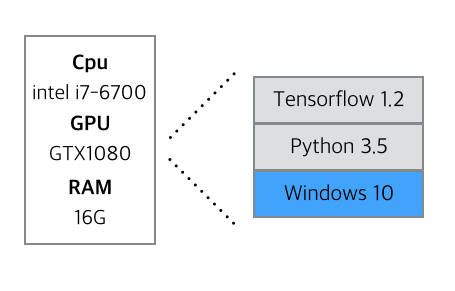
\includegraphics[width=0.3\textwidth]{fig/env.png}
  \end{center}
  \caption{Environment}
  \label{fig:xeon}
\end{figure}

\begin{figure*}[tb!]
    \centering
    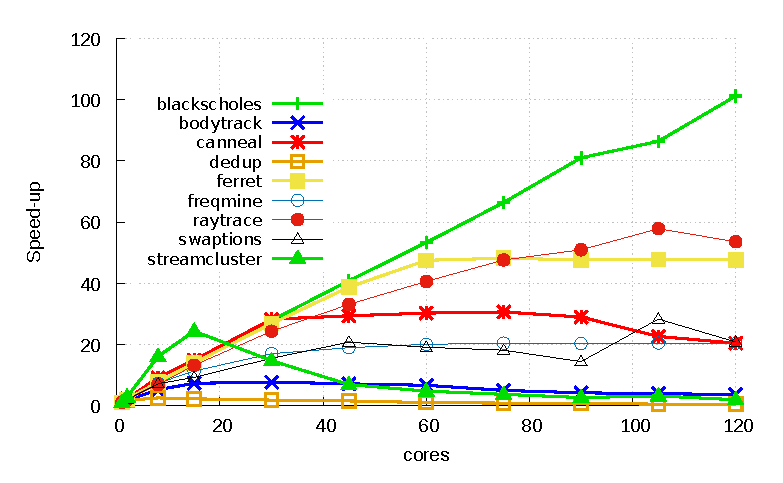
\includegraphics[width=4.8in]{graph/PARSEC.eps}
    \caption{벤치마크 실험 결과.}
    \label{fig:parsec}
\end{figure*}

For the measurement environment, software of the same version as Table ~\ref{tab:config} was used.
And the input data is collected by using the data that is open to the Internet.

\begin{table}[h!]
  \caption{Software version and input data}
  \centering
  \small
  \begin{tabular}{l l l l l} \toprule
    OS & Tool & Python & Tensorflow & input data\\
    \midrule
    Windows 10 & Tensorflow & 3.5.2 & 1.2.0 & fine dust data \\
    \bottomrule
  \end{tabular}
  \label{tab:config}
\end{table}


\section{ 설명}
본 연구에서는 PARSEC 벤치마크 중 9개의 벤치마크를 대상으로 측정을 하였다. 
각 워크로드의 설명과, 벤치마크에서 강조하고 있는 Data의 공유 정도 그리고
 락과 배리어등의 동기화 기법의 수에 대한 정보는  표~\ref{tab:workload}와 같다~\cite{parsecbench}.

\begin{table}[h!]
  \caption{워크로드 설명}
  \centering
  \scriptsize 
  \begin{tabular}{l l l l l} \toprule 
    워크로드명 &  & 데이터 공유 & 동기화 수 & 병렬화 모델\\
    \midrule
    blackscholes & 재정 분석 & 낮음 & 8 & data-parallel\\
    \midrule
    bodytrack & 컴퓨터 비젼 & 높음 & 2661 & data-parallel\\
    \midrule
    canneal & Engineering & 높음 & 34 & unstructured\\
    \midrule
    dedup & 엔터프라이즈 저장소 & 높음 & 160598 & pipeline\\
    \midrule
    ferret & 유사 검색 & 높음 & 345778 & pipeline\\
    \midrule
    freqmine & 데이터 마이닝 & 높음 & 990025 & data-parallel\\
    \midrule
    raytrace & 재정 분석 & 낮음 & 23 & data-parallel \\
    \midrule
    streamcluster & 데이터 마이닝 & 낮음 & 129918 & data-parallel\\
    \midrule
    swaptions & 재정 분석 & 낮음 & 23 & data-parallel \\
    \bottomrule
  \end{tabular}
  \label{tab:workload}
\end{table}

\section{워크로드 및 확장성 실험 결과}
 이번 장에선 본 연구는 두가지의 실험 결과를 바탕으로 결과를 도출해 내었다. 모든 실험은 15회 기준 평균 값으로 진행되었다.
첫번째로 각 프로그램마다 지정한 ROI가 프로그램의 확장성에 영향을 끼치는지를 확인하고 실험한 프로그램당 스레드별 실행시간을 기준으로 확장성을 확인해보았다.
\subsection{ROI (Region Of Interest)}
 먼저 ROI 부분이란 실제 병렬화되어서 실행되는 구간이다. 이 구간을 제외한 부분은 프로그램 실행시 필요한 초기화 부분이 대부분을 차지하고 있다. 표 ~\ref{tab:ROI_ratio}에서 확인할 수 있는 정적인 실행시간을 제외하고, ROI 부분만 확인 하였을때 모든 프로그램에서 최대 스레드 x0.7 수준의 성능향상이 있었다. 이로 비추어 볼때 실제로 우리가 측정하는 ROI시간들이 프로그램의 성능을 측정한다고 볼 수 있다.
\begin{table}
\caption{비 ROI 실행 시간} 
\label{tab:ROI_ratio}
\centering
\begin{tabular}{c|c|c}
\hline
워크로드 명 & 평균 실행시간 (s) & 전체 대비 비(\%) \\ \hline
blackscholes & 21.23 & 12.3 \\ \hline
bodytrack & 0.10 & 0.2 \\ \hline
canneal & 47.37 & 8.7 \\ \hline
dedup & 0.74 & 2.7\\ \hline
ferret & 0.18 & 0.1\\ \hline
freqmine & 0.08 & 0.1\\ \hline
raytrace & 59.52 & 25.9\\ \hline
streamcluster & 0.01 & 0.1\\ \hline
swaptions & 0.01 & 0.1\\ \hline
\end{tabular}
\end{table}
\subsection{실험 결과}
해당 실험결과는 native 입력 데이터셋을 기준으로 스레드 숫자를 늘려가며 기대하는 선형적인 확장성을 보여줄 수 있는지 확인한 결과이다. 가장 좋은 결과를 보여준 blackscholes 를 제외하고 A,B 그룹 2가지로 나누어서 결과를 유추할 수 있다.
\begin{itemize}
\item \textbf{blackscholes} :
해당 프로그램의 비 ROI 실행 시간은 대부분을 입력 값을 초기화하는 곳에 사용한다. 또한 표 ~\ref{tab:workload} 에서 확인 할 수 있듯이 동기화와 데이터 공유의 빈도가 매우 낮다. 이로 인해서 완벽한 선형은 아니지만 다른 8개의 벤치마크에 비해서 가장 높은 멀티스레딩 대비 확장성을 보여준다.
\item \textbf{A 그룹} (bodytrack,canneal,dedup,ferret,freqmine) : 해당 그룹에 속하는 프로그램들은 모두 동기화와 데이터 공유의 빈도가 매우 높다. 결과도 성능이 비교적 완만하게 증가하다가 오히려 10~20 스레드 사이에서부터 성능의 하락이 일어나고 있다. 따라서 측정된 프로그램들 중 가장 확장성이 낮은 그룹이라고 볼 수 있다.
\item \textbf{B 그룹} (streamcluster,raytrace,swaption) : 해당 그룹에 속하는 프로그램들은 동기화 빈도는 높지만 데이터공유의 정도가 낮은 그룹이다. 그림 ~\ref{fig:parsec} 에서 그룹 B 에 속해있는 프로그램들의 그래프를 살펴보면, 오히려 스레드 숫자가 50개 정도일 때 까지는 선형적인 확장성을 보이고 있다. 심지어 streamcluster 의 경우 스레드가 낮을때에 국한해서 blackscholes 의 확장성을 훨씬 웃돌고 있다. 하지만 모두 일정 스레드 이후에는 성능이 더이상 증가하고 있지 않다.
\end{itemize}

\begin{table}[]
\centering
\caption{결과그룹}
\label{tab:result_group}
\begin{tabular}{|c|c|}
\hline
\multicolumn{2}{|c|}{데이터 공유}                                                                                                                                         \\ \hline
높음                                                                                   & 낮음                                                                            \\ \hline
\begin{tabular}[c]{@{}c@{}}bodytrack,dedup,canneal\\ ferret,freqmine(A)\end{tabular} & \begin{tabular}[c]{@{}c@{}}streamcluster\\ raytrace,swaptions(B)\end{tabular} \\ \hline
\end{tabular}
\end{table}
\section{결론 및 향후 연구}

PARSEC의 ROI 부분만 측정하여 분석한 결과 PASEC의 대부분의 워크로드는 확장성에 문제를 
가지고 있다. 특히 표 ~\ref{tab:result_group}의 그룹 A와 B 를 비교해보았을때 데이터공유 문제가 스레드가 많아지면 많아질 수록 부각 되는 것을 확인할 수 있었다.  PARSEC은 공유 메모리 기반의 멀티 쓰레드를 이용한 워크로드로 구성되어 있는 벤치마크이다.
향후 연구로는 본 연구의 결과를 이용하여 리눅스의 매니코어 시스템에서 멀티 쓰레드의 
문제점을 분석할 예정이다.

\bibliographystyle{ieeetr}
\begin{thebibliography}{7}
\bibitem{Etri}
정진환, 김강호, 김진미, 정성인. 
\newblock Manycore 운영체제 동향. 
\newblock 전자통신 동향 분석 29권 5호, 2014. 
\bibitem{kesl1}
경주현, 임성수.
\newblock 매니코어 시스템을 위한 리눅스 가상 메모리 관리의 락 경합 분석. 
\newblock 한국정보과학회, 한국정보과학회 학술발표논문집 , 2015.6, 1571-1573, 2015
\bibitem{kesl2}
경주현, 윤성민, 임성수.
\newblock 매니코어 환경에서 로그 기반 동시적 업데이트 기법을 활용한 리눅스 커널 확장성 개선.
\newblock 한국정보과학회 학술발표논문집 , 2016.12, 512-513, 2016
\bibitem{AustinTClements2012RCUBalancedTrees}
Austin~T. Clements, M.~Frans Kaashoek, and Nickolai Zeldovich.
\newblock Scalable address spaces using {RCU} balanced trees.
\newblock In {\em Architectural Support for Programming Languages and Operating
  Systems (ASPLOS 2012)}, pages 199--210, London, UK, February 2012.
\bibitem{parsecbench}
Bienia, Christian and Kumar, Sanjeev and Singh, Jaswinder Pal and Li, Kai
\newblock The PARSEC benchmark suite: characterization and architectural
implications.
\newblock PACT '08 Proceedings of the 17th international
conference on Parallel architectures and compilation techniques Pages 72-81 . 2008.
\bibitem{Clements2013RadixVM}
Austin~T. Clements, M.~Frans Kaashoek, and Nickolai Zeldovich.
\newblock Radixvm: Scalable address spaces for multithreaded applications.
\newblock In {\em Proceedings of the 8th ACM European Conference on Computer
  Systems}, EuroSys '13, pages 211--224, New York, NY, USA, 2013.

\end{thebibliography}

%\bibliographystyle{ieeetr}
%\bibliography{ref}

\end{document}
